\documentclass[letter]{article}
\usepackage{microtype}
\usepackage{fullpage}
\usepackage{url}
\usepackage{graphicx}
\usepackage{float}
\usepackage{caption}

\title{\\
  Computer Science Department\\
  Ball State University\\
  Technical Report 2017--01}

\author{
  Chas Busenburg
  \and
  Paul Gestwicki
  \and
  Ying Liu
  \and
  Jacob Rendall}

\begin{document}

\begin{centering}
{\Large A requirements and design analysis for an interactive online donation interface}\\
\vspace{0.5cm}
Chas Busenburg, Paul Gestwicki\footnote{Corresponding author}, Ying Liu, and Jacob Rendall\\
Computer Science Department\\
\texttt{cwbusenburg@bsu.edu}, 
\texttt{pvgestwicki@bsu.edu},
\texttt{yliu12@bsu.edu},
\texttt{jbrendall@bsu.edu}\\
\vspace{0.5cm}
\today\\
\vspace{0.5cm}
Computer Science Department\\
Ball State University\\
Technical Report 2017--01\\
\end{centering}

\section*{Introduction}

% I wonder if we should start with something more clear than the background,
% to say what the big picture is. Something like, "In Spring 2017,
% our team worked to design and develop a novel interactive donation
% system for ecoREHAB...".

ecoREHAB is a nonprofit organization in Muncie, Indiana, that specializes
in environmentally-friendly, economically-sound rehabilitation of houses.
The organization started as an immersive learning project at Ball
State University in 2009, as a collaboration between the 
City of Muncie Department of Community Development and the 
Ball State College of Architecture and Planning.
ecoREHAB was successful enough to become an independent non-profit, 
although it maintains partnerships with the university.
Their mission statement is given below.

\begin{quote}
  Our Mission is to provide leadership in ecologically sound and
  sustainable rehabilitation of existing housing and
  neighborhoods. ecoREHAB of Muncie, Inc. will engage in activities
  that include: 1)~acquisition and ecologically sustainable
  rehabilitation of affordable housing; 2)~provide resources to aid
  homeowners and in rehabilitation of existing housing following
  sustainable design, material and system strategies; and 3)~other
  activities relative to housing that help the community to achieve
  the triple-bottom-line of economic prosperity, environmental
  protection, and social equity.
\end{quote}

% Actual first name: Katherine
In Spring 2017, Kate Elliott led an undergraduate team of journalism,
marketing, and public relations students in a new immersive learning
partnership with ecoREHAB, with the goal of revising the organization's
branding and Web presence.
ecoREHAB has been primariliy grant-funded, and one of the 
goals for the revised Web site was to accept donations from
the community, including local residents and university alumni.

% Use '\ ' to indicate that the '.' does not end a sentence, 
% as in, "Dr.\ Paul Gestwicki". This will fix the spacing error
% in the output PDF
% The course is "requirements and design" of course.
% Use '~' for nonbreaking spaces, e.g. between the "CS" and "691" here,
% to ensure they don't show up on separate lines.
As a part of Dr. Paul Gestwicki's research and design course (CS 691)
at Ball State University, a collaborative effort was established with
% First name is not appropriate here. "Ms.\ Elliott" or simply "Elliott"
% would be appropriate.
Kate's class. 
% An initiative is not "on" something, it simply "is" something.
Their main initiative was on the re-branding process for
ecoREHAB while the donation system for the organization was the
% I would probably just use "CS691", but if you want the space,
% make it non-breaking (~)
primary focus for our CS 691 course. The aim of this project was to
design and develop an interactive donation system for ecoREHAB, with
% There's confusion here between _our_ aim and the learning goal _of the 
% end users of the product_. This merits expansion and explanation.
the main learning goal from the interaction being given below.

% This is too short to merit a blockquote. Single-line quotations
% should just be given in-line.
\begin{quote}
	Houses can be rehabbed in an environmentally-friendly way, although it takes resources (time, money, knowledge). 
% Parenthetical phrases are bad. Let's make it clearer.
\end{quote}

This report presents the design process used by our class for the
donation system.
% Yes. Let's say more. What was our timeline? This paragraph should 
% contextualize all that follows this section. 
% At a higher level, one-sentence paragraphs are always a sign of
% an incomplete document. They may state something that has already
% been said, in which case they are eliminated as redundant;
% they may introduce a new idea, in which case they need expansion
% in the paragraph; or they may reinforce an existing idea, in which
% case they belong in an existing paragraph.

\section*{Design}
% What do you mean by "a primary component" here?
Donation systems are a primary component for raising funds for
nonprofit organizations. 
Though a donation system can be as simple as
having a user input a monetary value and then payment information,
this is not the way our group originally approached developing the
system for ecoREHAB. 
% Yes, but why not? Give the design context and criteria, or weave it
% into the client meetings discussion below.
The first step that was taken involved meeting
with both ecoREHAB board members 
% Who? This is the first time this concept has been introduced                  
and Kate to discuss their ideas on
how they would like donations to be processed and accepted. From this
initial meeting, several key points were made that would go on to
serve as a foundation for how we believed the donation system should
function and appear like to users. 
% "A few ... included", it's just not a very strong claim. Let's
% make it clearer what's going on here.
% We can, and should, use nomenclature of requirements to describe these.
A few major points from this
meeting included the following:
\begin{itemize}
	\item{Show different categories involved in building a house.}
	\item{Give user eco-friendly information when a category is selected.}
	\item{Interactive "house" or display to allow user to select type/amount of donation.}
\end{itemize}
Using these concepts, our team's next step was to identify a process to implement the ideas.
% Nope. Next step was to build a story map! Or maybe it was something else,
% but it certainly wasn't jumping into implementation.

% Because of the revision needed above, of course this paragraph
% will have to change.
In order to complete a design of the desired ecoREHAB donation system,
our process began with drawing sketches of how a potential donation
page would look. At this point we were aware that Kate and her team
had acquired the Pena 
% Tilde over the n: \~{n}
% Also, what _is_ the Pena theme? Why is it important? What's a theme,
% for that matter?
Wordpress theme to develop the new website for
ecoREHAB, so our implementation for the donation system would be
integrated into this website. Different members of our team drew a
variety of preliminary design sketches to be evaluated. Several of
these basic designs are shown below in Figures
% You have a hyphen below where you want an en-dash: --
\ref{fig:1}-\ref{fig:3}.
\begin{figure}[H] % Why specify H? I say, let LaTeX do its thing.
	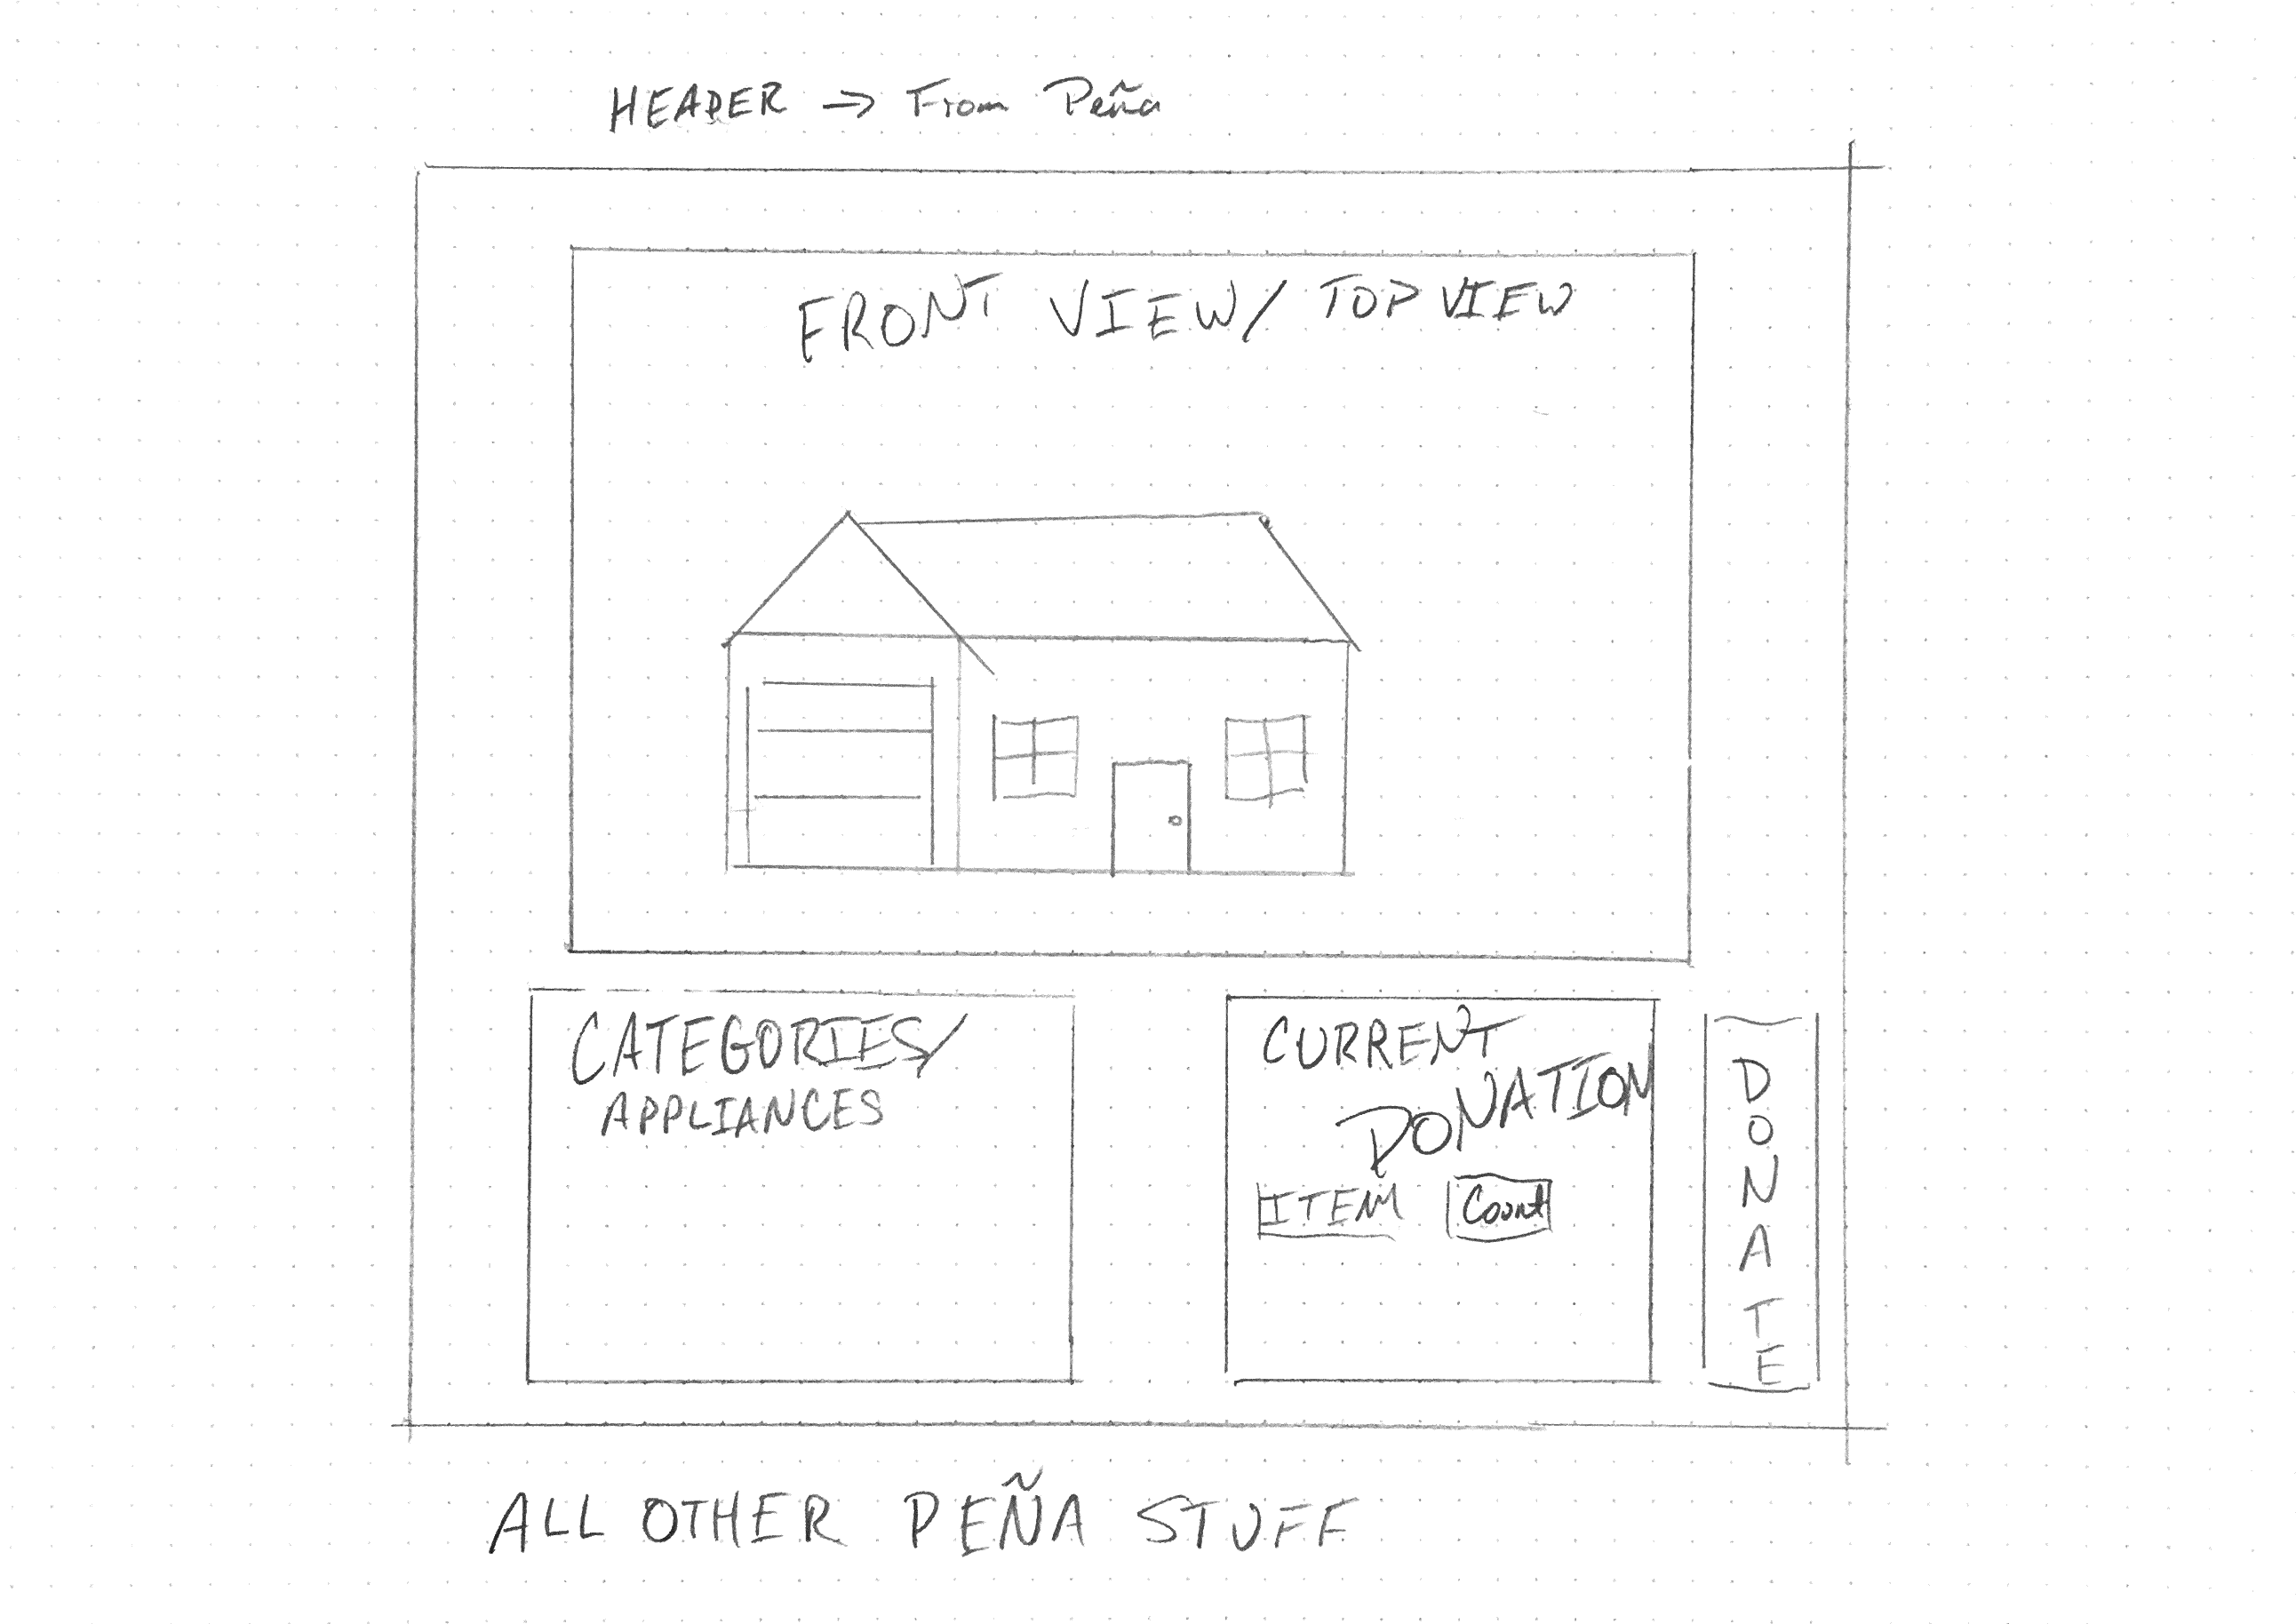
\includegraphics[width=15cm, height=10cm]{example}
	\captionsetup{justification=centering}
	\caption{A basic example of a donation page.}
	\label{fig:1}
\end{figure}
\begin{figure}[H]
	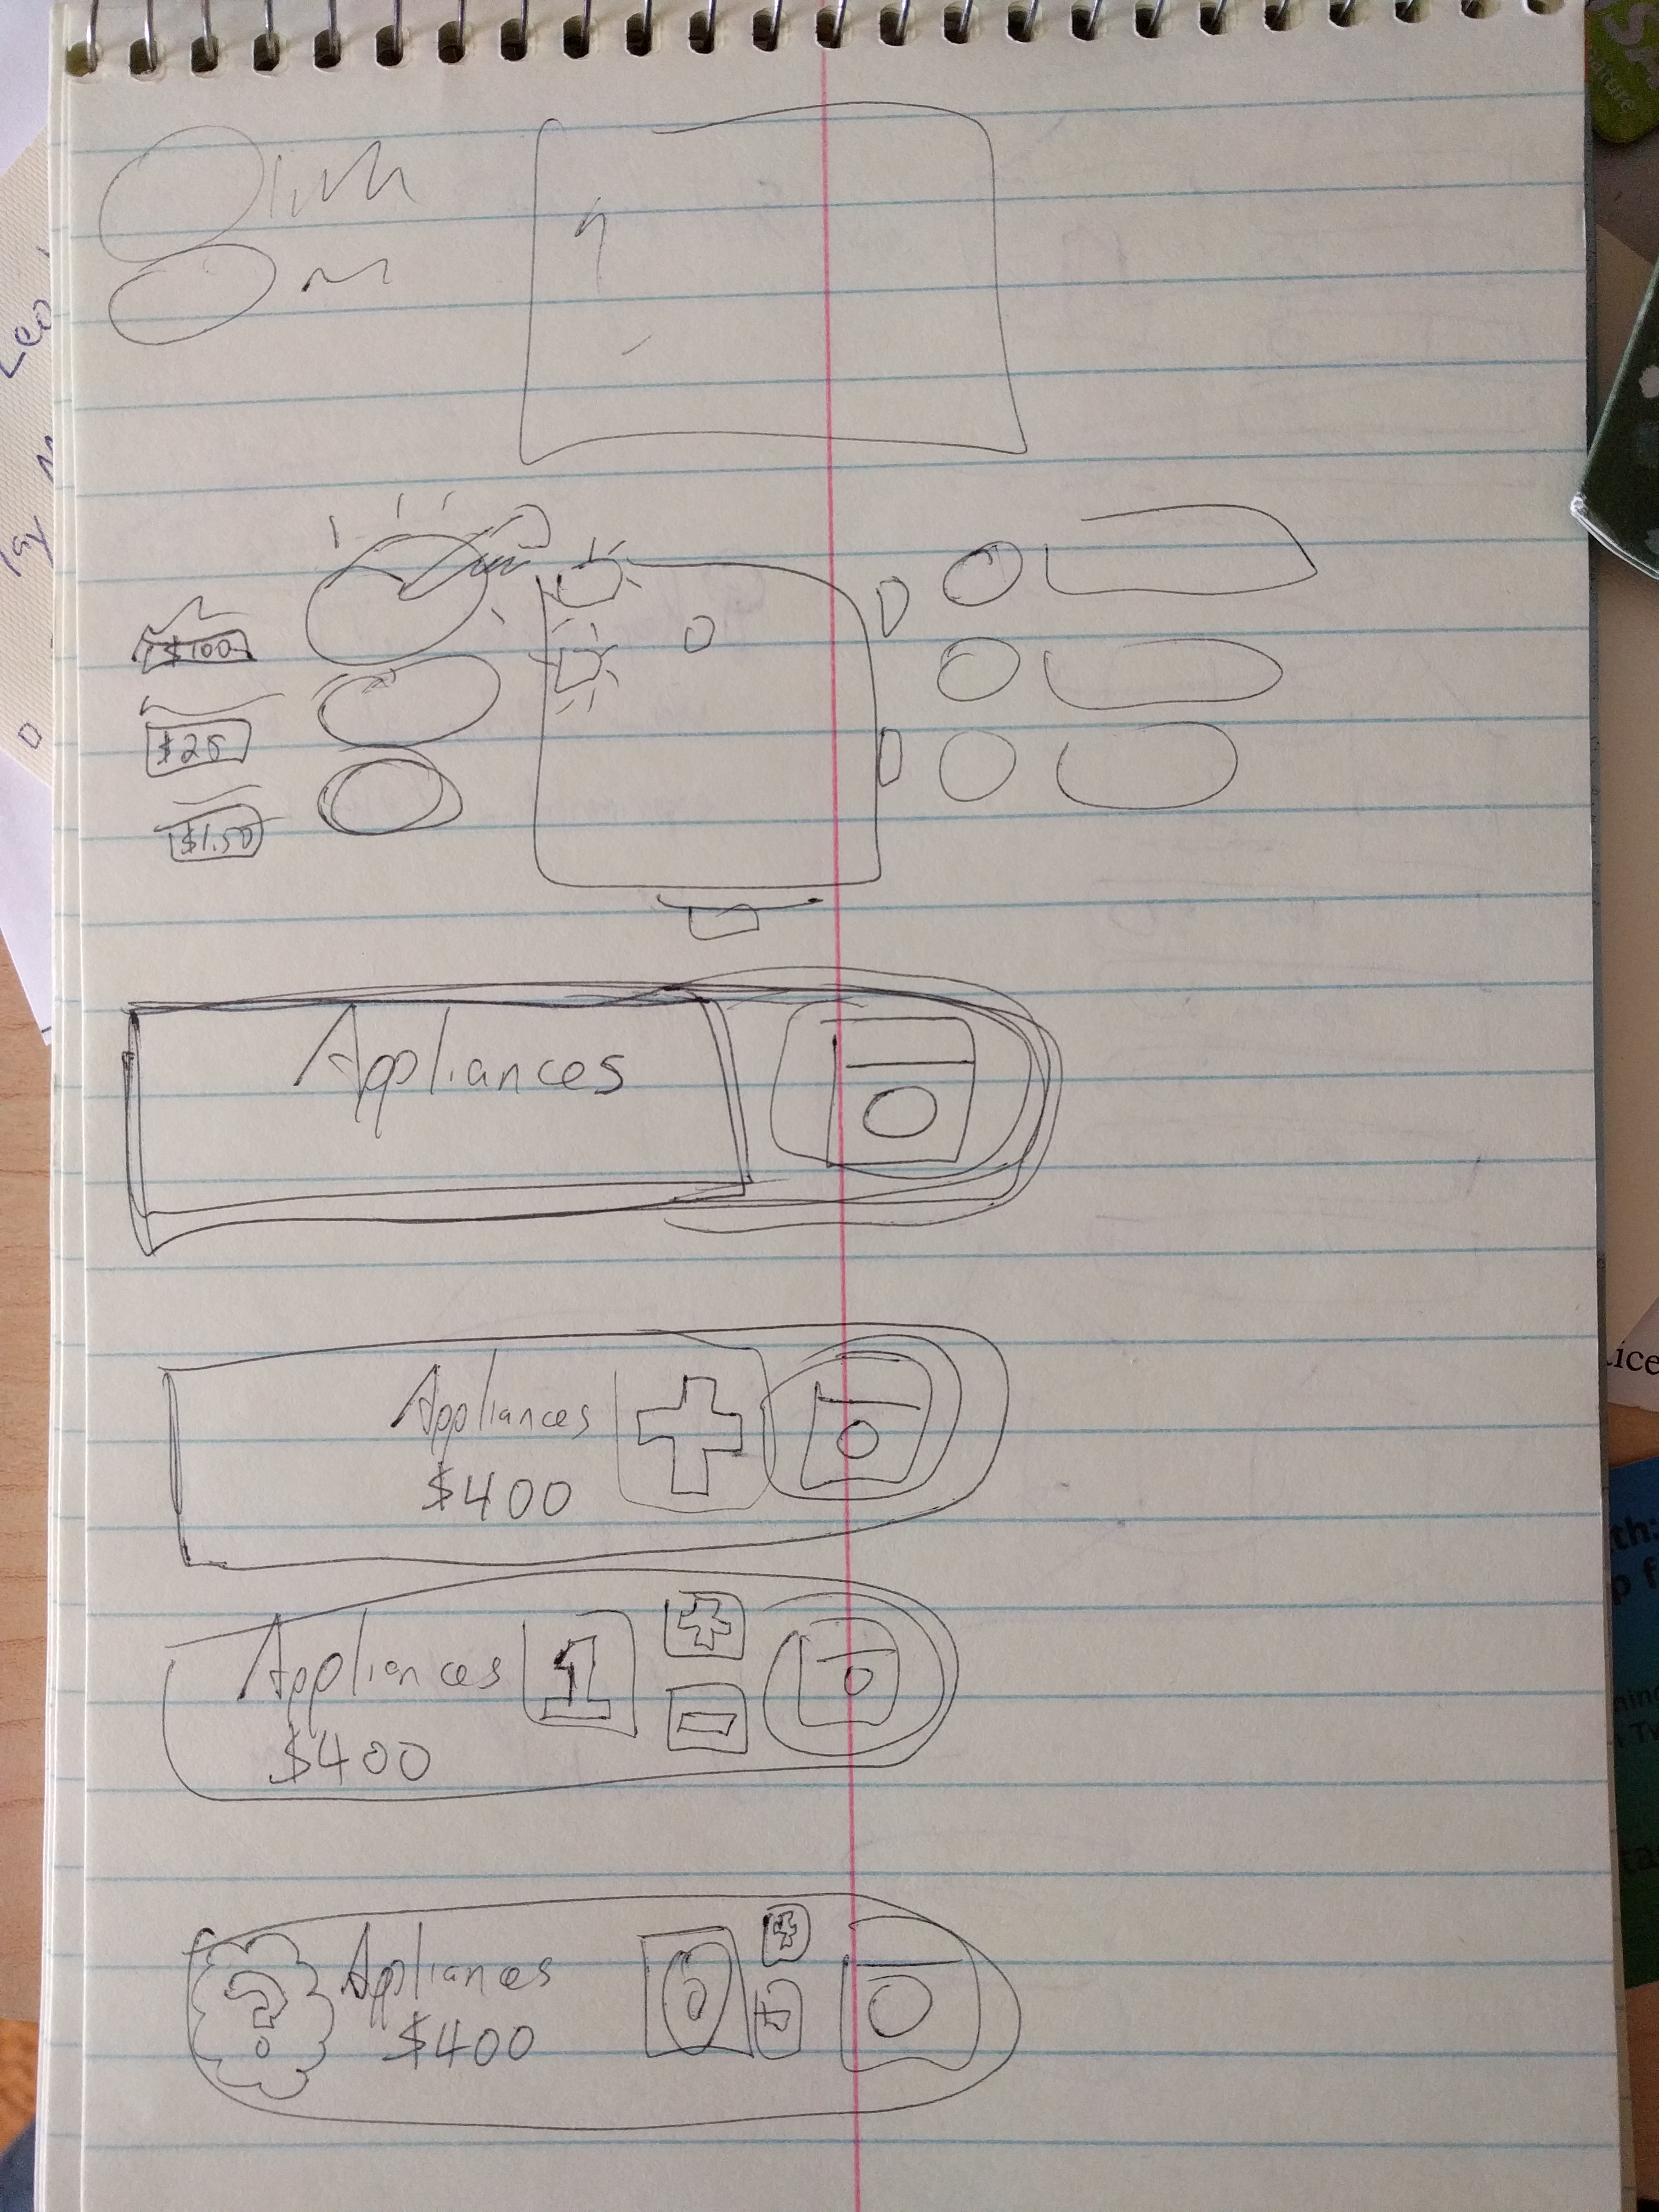
\includegraphics[width=7cm, height=9cm]{Example4}
	\captionsetup{justification=centering}
	\centering
	\caption{A donation page with unique symbols to identify the different categories.}
	\label{fig:2}
\end{figure}
\begin{figure}[H]
	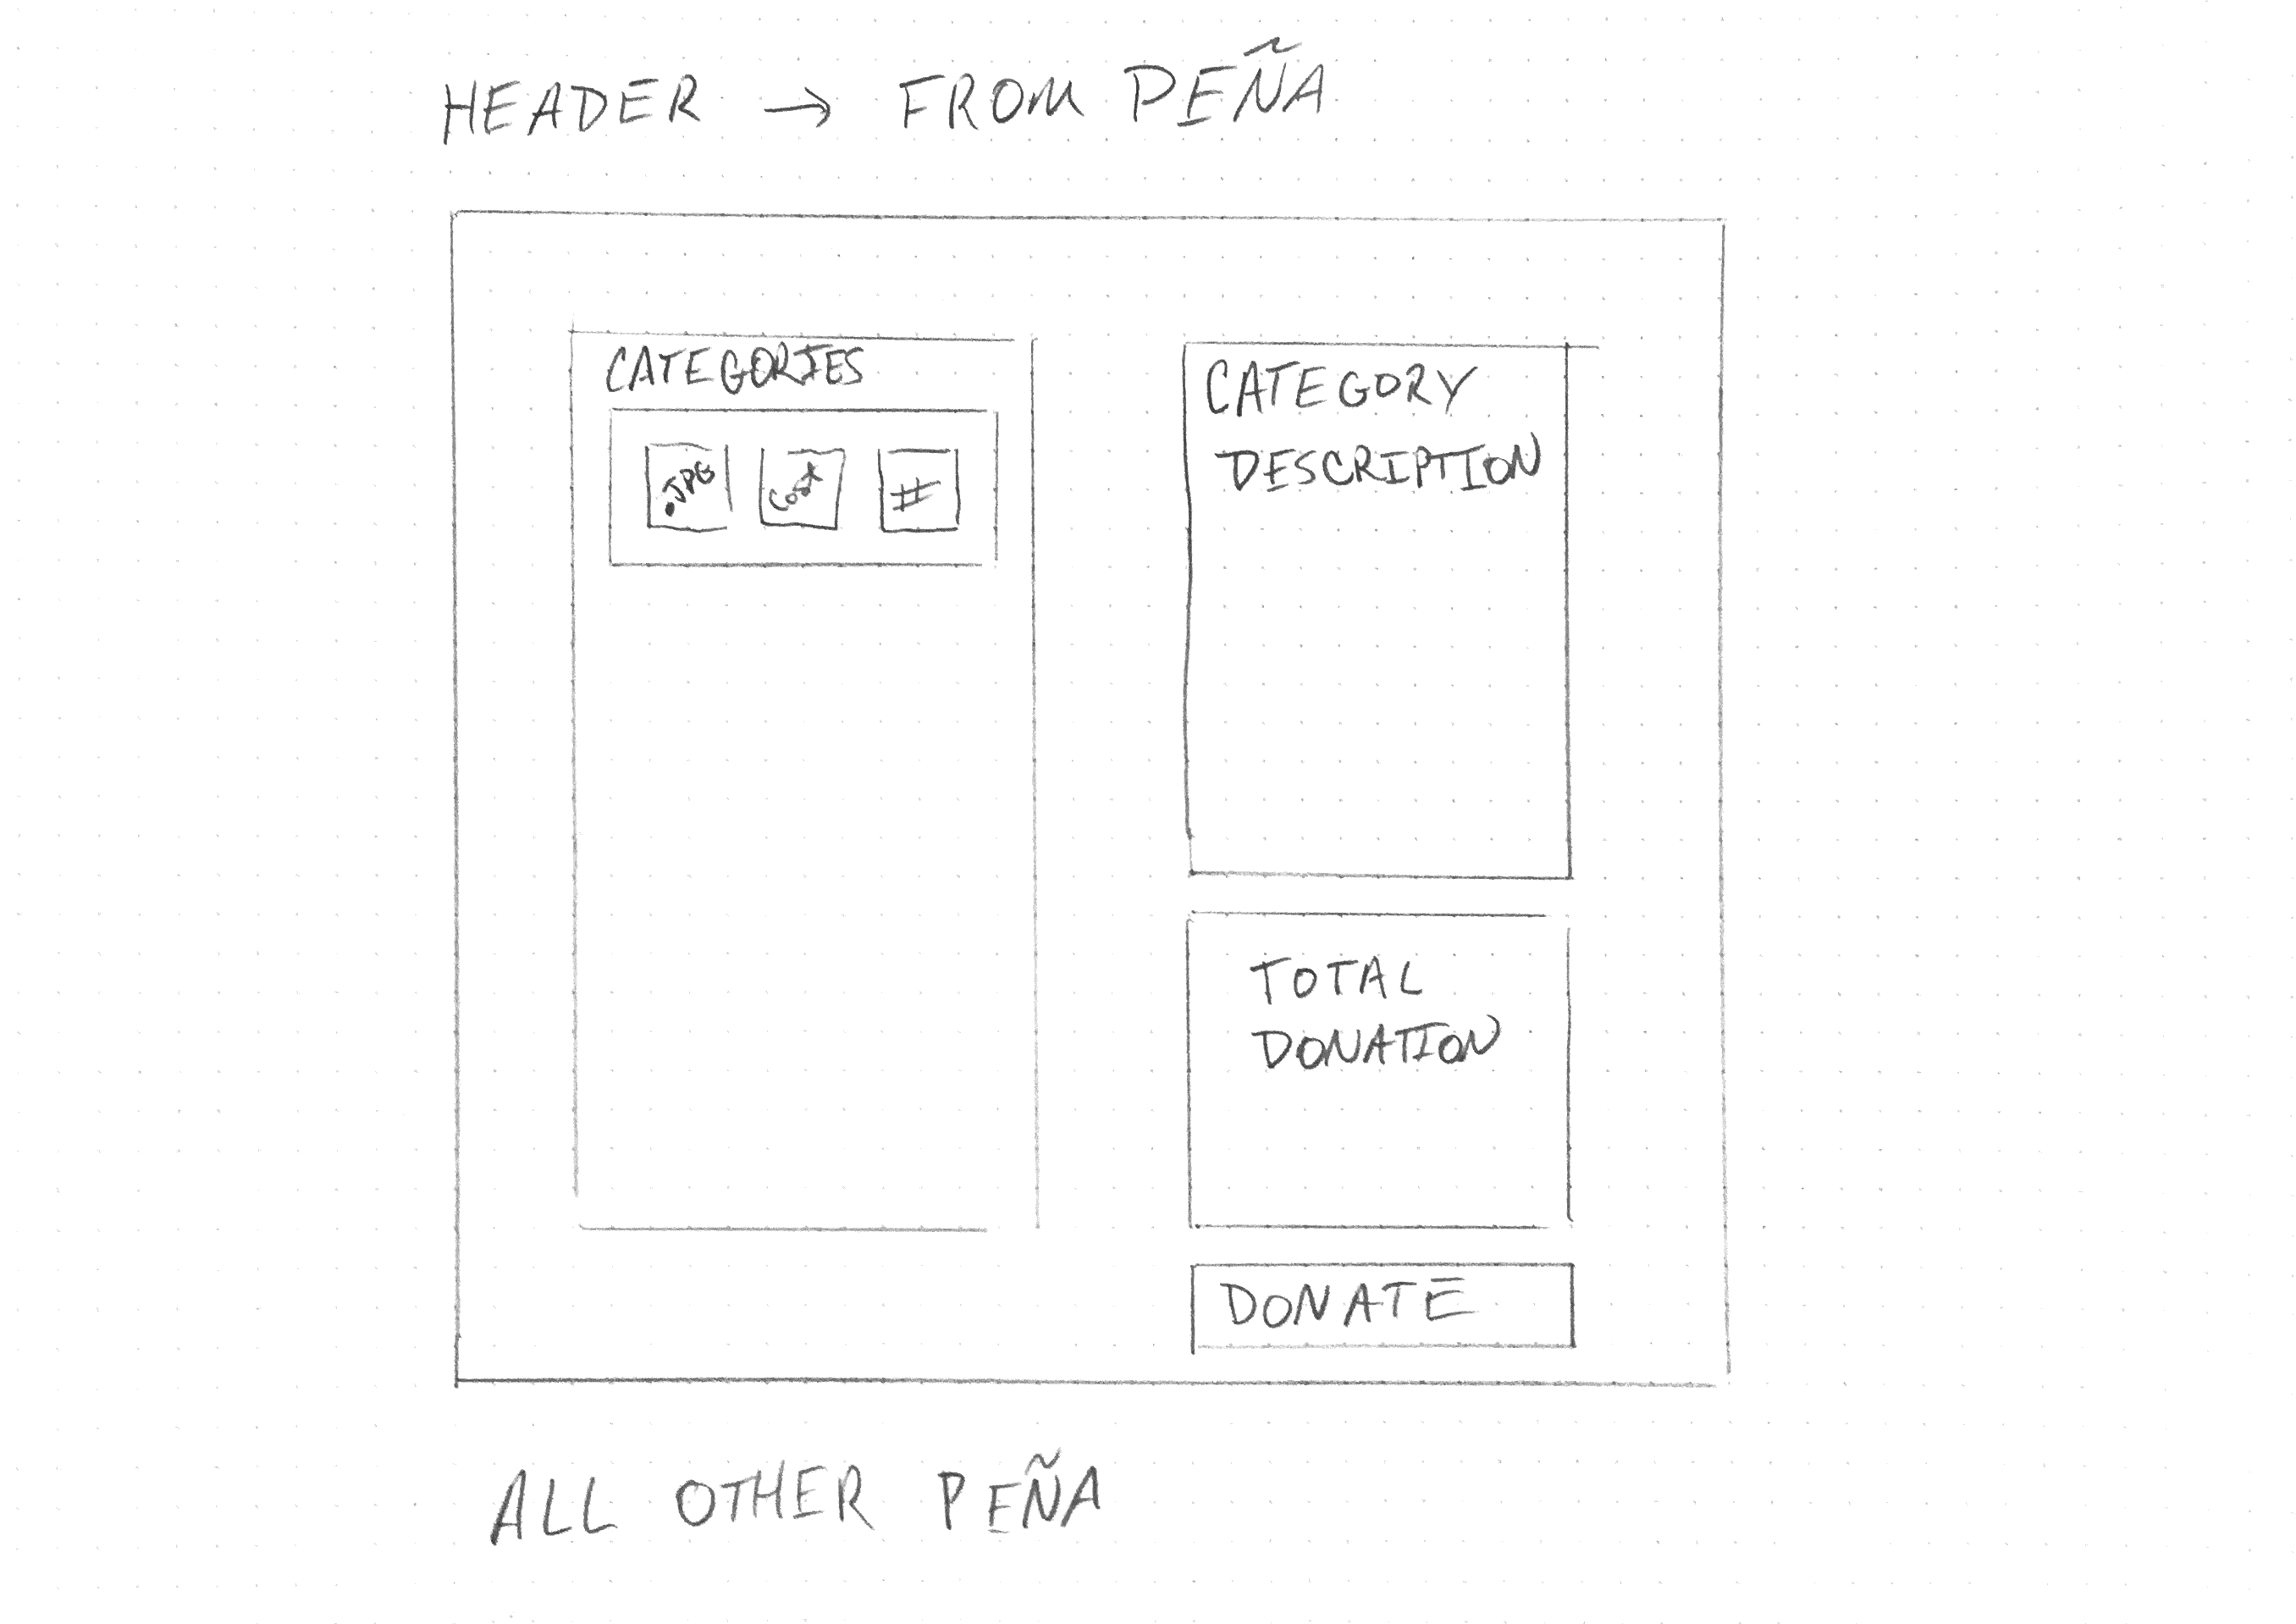
\includegraphics[width=10cm, height=10cm]{Example5}
	\captionsetup{justification=centering}
	\centering
	\caption{A simple donation page that incorporates the ability \\ to view more information about each category.}
	\label{fig:3}
\end{figure}

% This strikes me as too narrative, like a personal journal or analytic
% memo rather than a tech report. 
Once we had these basic sketches in hand, our team debated which
features were good and/or necessary as well as those deemed to be out
of the scope of the project. From his discussion, it was determined
that the points of emphasis that would need to be implemented on the
donation page included showing the different categories involved with
building a house, a short description of each category, and adding to
the donation based on an amount within a category. Since the original
idea was to create an interactive experience for when the user makes a
donation, we determined that the interactivity would be a result from
clicking on a category's symbol, resulting in the information display
as well as highlighting a portion of a house related to the
category.
 Before attempting to implement this design, we developed a
paper prototype to test its effectiveness. 
% A paper prototype is an implementation---a prototypical one.
% The prototype was important: is this really all you want to say about it?
% The explanation provided in the appendix, it's a write-only explanation:
% it makes sense to us, but I don't think it frames the prototype 
% appropriately for a reader who cannot hold it or have us explain it.
The prototype our team
created can be viewed in the Appendix.

% So the real focus of this paper should be our design, the design of
% a novel interactive donation system, but this is almost entirely
% omitted here, in favor of a narrative about us. The reader doesn't
% care about _us_; the reader cares about _it_.

After testing the paper prototype internally, we needed some external
validation before moving towards implementing the system we had
designed. During a meeting with Kate, she was able to test our
prototype and provide feedback. This feedback included both how she
thought the prototype worked and her thoughts on how the donation page
may need to appear on the website. From this meeting, our team
determined that, although the interactivity element for ecoREHAB's
donations is interesting, it feel out of the scope of our project due
to time constraint and lack of experience with graphic design. At this
point in the process, we determined that a basic donation page was
needed, which included information and/or prompts about donating to
ecoREHAB and buttons to input the donation amount for a user.

% I don't think any of this from here below needs to be in the tech
% report. This is just what we did in the course, which is not of 
% archival value. Every course could write a paper about what they
% did, but our work is already manifest in the ecoREHAB site;
% what is not manifest is all the work we did on the other design---and
% hence the purpose for a TR.
With a new look at how the donation page needed to function, our team
began to develop a web page that would include only text and donation
buttons. We developed this donation page using HTML and
AngularJS. After implementing a new aspect of the donation page, we
tested it by loading the web page into our development environment,
which included the Pena theme being used by Kate's team on the new
ecoREHAB website. One aspect of doing a donation page that came into
play at this point was how to process the donations. We determined
that using a third party software would be best, so we set a PayPal
account that would process all the donations. The donation buttons
were made to take the user to PayPal to finish paying for the
donation, and upon completion the user was then returned to the
ecoREHAB website.

After thoroughly testing the donation page we developed, the last step
in the process was to add the page onto Kate's website. At this point
we ran into a major problem. While testing, we had been using a
Wordpress.org environment, whereas Kate's team had been working in a
Wordpress.com environment. We found out that Wordpress.com does not
allow for JavaScript to be used. Thus, the donation button, which was
developed using AngularJS, could not work. After diagnosing the
problem, we were able to do a workaround by making buttons that
% Parenthetical phrases are usually indications of a "spoken word"
% approach, but in writing, we have the space to clarify that.
% We don't have to interrupt a sentence: we can make a whole new one,
% or a footnote, or an endref, etc.
Wordpress.com allowed (using \url{<https://dabuttonfactory.com>}) to
include the redirection from the ecoREHAB site to PayPal so donations
could be completed. A small glimpse of how the donation page turned
out is shown below in Figure \ref{fig:4}.
\begin{figure}[H]
	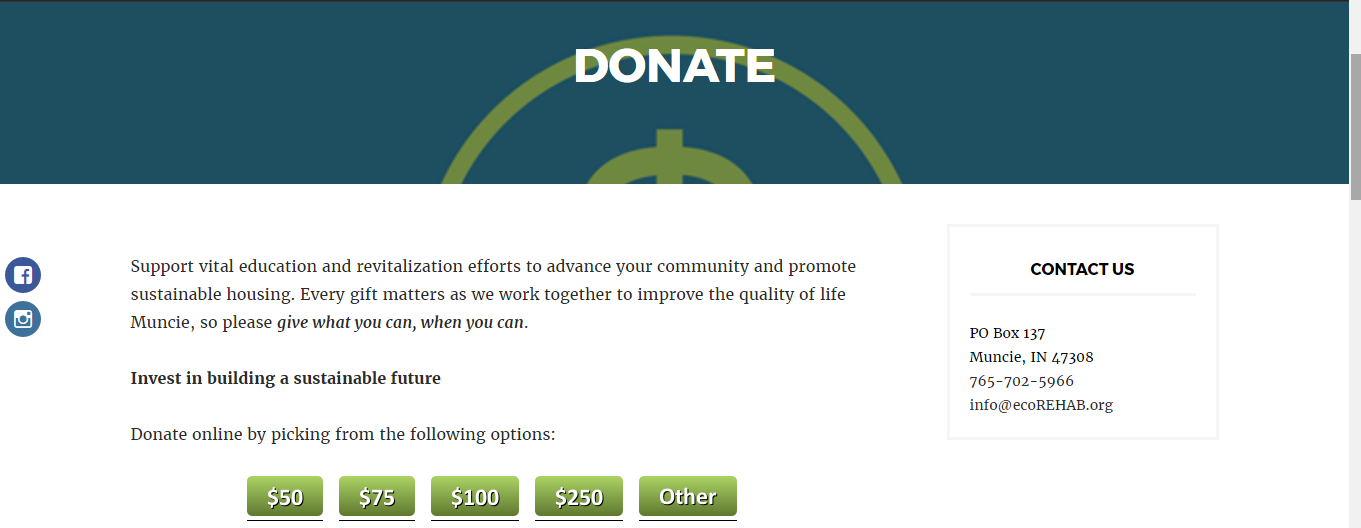
\includegraphics[scale=0.5]{Donation}
	\captionsetup{justification=centering}
	\centering
	\caption{Part of the donation page developed by our team.}
	\label{fig:4}
\end{figure}
The final donation page we created can be found on Kate's website at \url{<https://loveandtruthiness.wordpress.com/donatevolunteer/donate/>}.

\section*{Conclusions and Future Work}
The design process of the donation system for the non-profit
organization ecoREHAB has been presented in this report. After
developing several different preliminary designs for the donation web
page were made, the main aspects for the interactive element of the
system were established. These included clickable category symbols
that would allow users to view extra eco-friendly information about
the selected category. After testing this interactive element,
although deemed useful, it was determined that with that this
component could not be comleted due to a lack of certain graphic
design skills and the time remaining to the project's due date. The
interactivity was also not necessary for the donation system to
function. This led to our team creating a simple donation system using
buttons that the user can interact with when attempting to donate to
ecoREHAB.

In the future, this interactive donation system can easily be
implemented as described in this report. The team completing this task
will need some graphic design experience in order to ensure high
quality of the interactive images. Beyond what has been described,
another potential avenue for donation interactivity is to keep
progress of the donations coming in. In the context of building a
house, progress could include the donation amount that has already
been put towards a house and the remaining amount of money needed to
complete the project. An design example of such a system is shown in
Figure \ref{fig:5}.
\begin{figure}[H]
	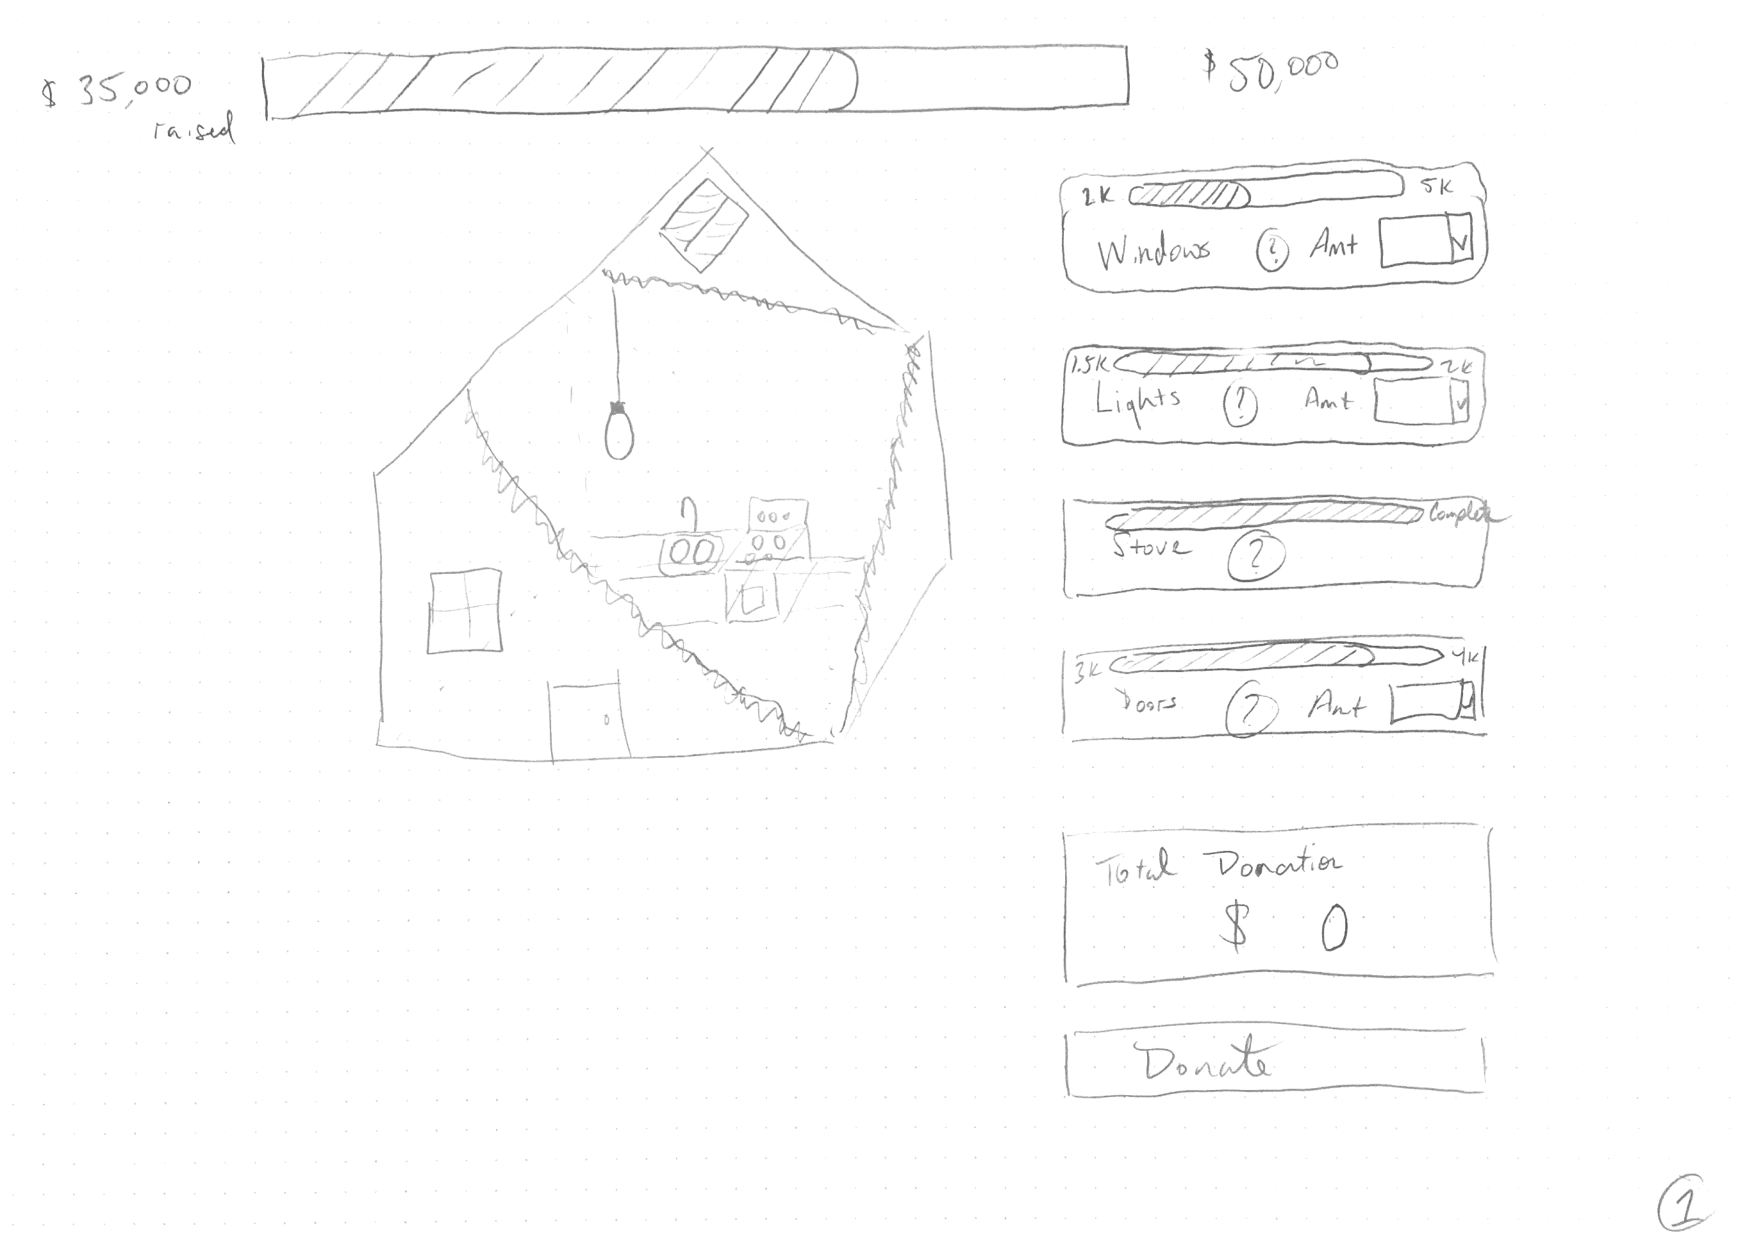
\includegraphics[page=1, scale=0.5]{Example3}
	\captionsetup{justification=centering}
	\centering
	\caption{Design that included progress bars towards the total amount needed to build a house.}
	\label{fig:5}
\end{figure}
\section*{Appendix}
\begin{figure}[H]
	\includegraphics[page=1, scale=0.75]{PaperPrototype}
\end{figure}
\begin{figure}[H]
	\includegraphics[page=2, scale=0.75]{PaperPrototype}
\end{figure}
\begin{figure}[H]
	\includegraphics[page=3, scale=0.75]{PaperPrototype}
\end{figure}
\begin{figure}[H]
	\includegraphics[page=4, scale=0.75]{PaperPrototype}
\end{figure}
\begin{figure}[H]
	\includegraphics[page=5, scale=0.75]{PaperPrototype}
\end{figure}
\begin{figure}[H]
	\includegraphics[page=6, scale=0.75]{PaperPrototype}
\end{figure}

\end{document}
